\subsection{Prodotto realizzato}
\label{subsec:prodotto-realizzato}

La {\hyperref[fig:login]{Figura 3.6}} mostra la pagina di \textit{login}, che consente agli utenti di accedere inserendo le proprie credenziali.\\
In caso di problemi, è disponibile un'opzione per reimpostare la \textit{password} cliccando su "\textit{Password} dimenticata".
\begin{figure}[H]
    \centering
    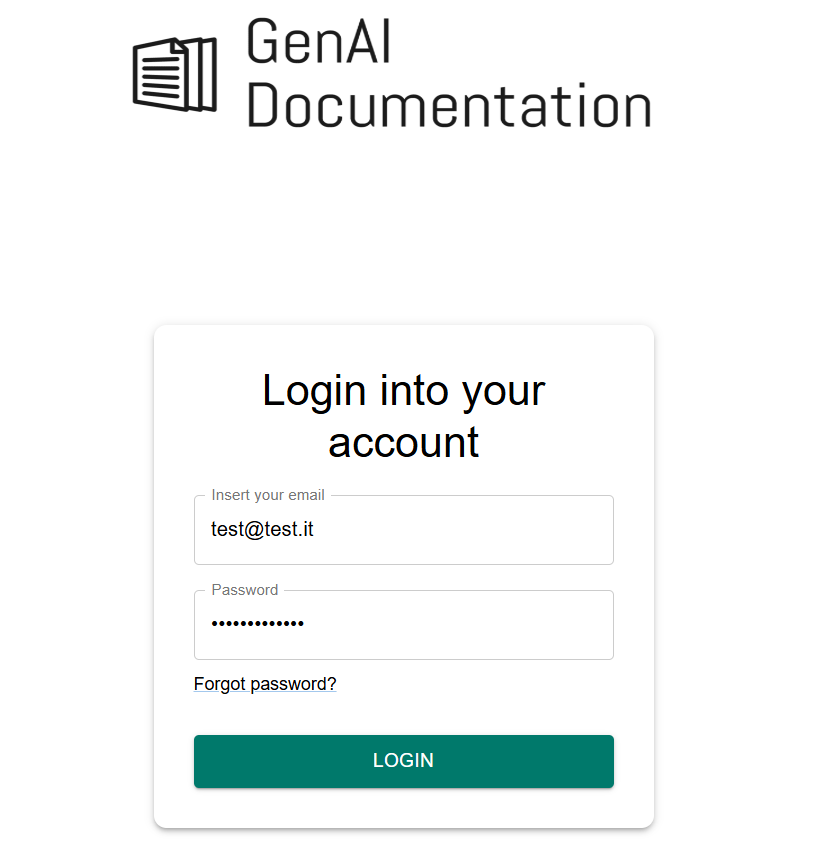
\includegraphics[width=1\textwidth]{applicazione/login.png}
    \caption{Schermata di \textit{login} del progetto}
    \label{fig:login}
\end{figure}

\pagebreak
\noindent La {\hyperref[fig:dashboard]{Figura 3.7}} mostra la \textit{dashboard}, che offre una panoramica dei progetti generati in precedenza e delle bozze di progetto, con la funzionalità, sia per progetti che per le bozze,
di cercarle per nome o filtrarle per data. \\
Da questa pagina, gli utenti possono accedere ai dettagli di un singolo progetto o iniziare la generazione di un nuovo progetto, oltre che effettuare il \textit{logout}.\\
\begin{figure}[H]
    \centering
    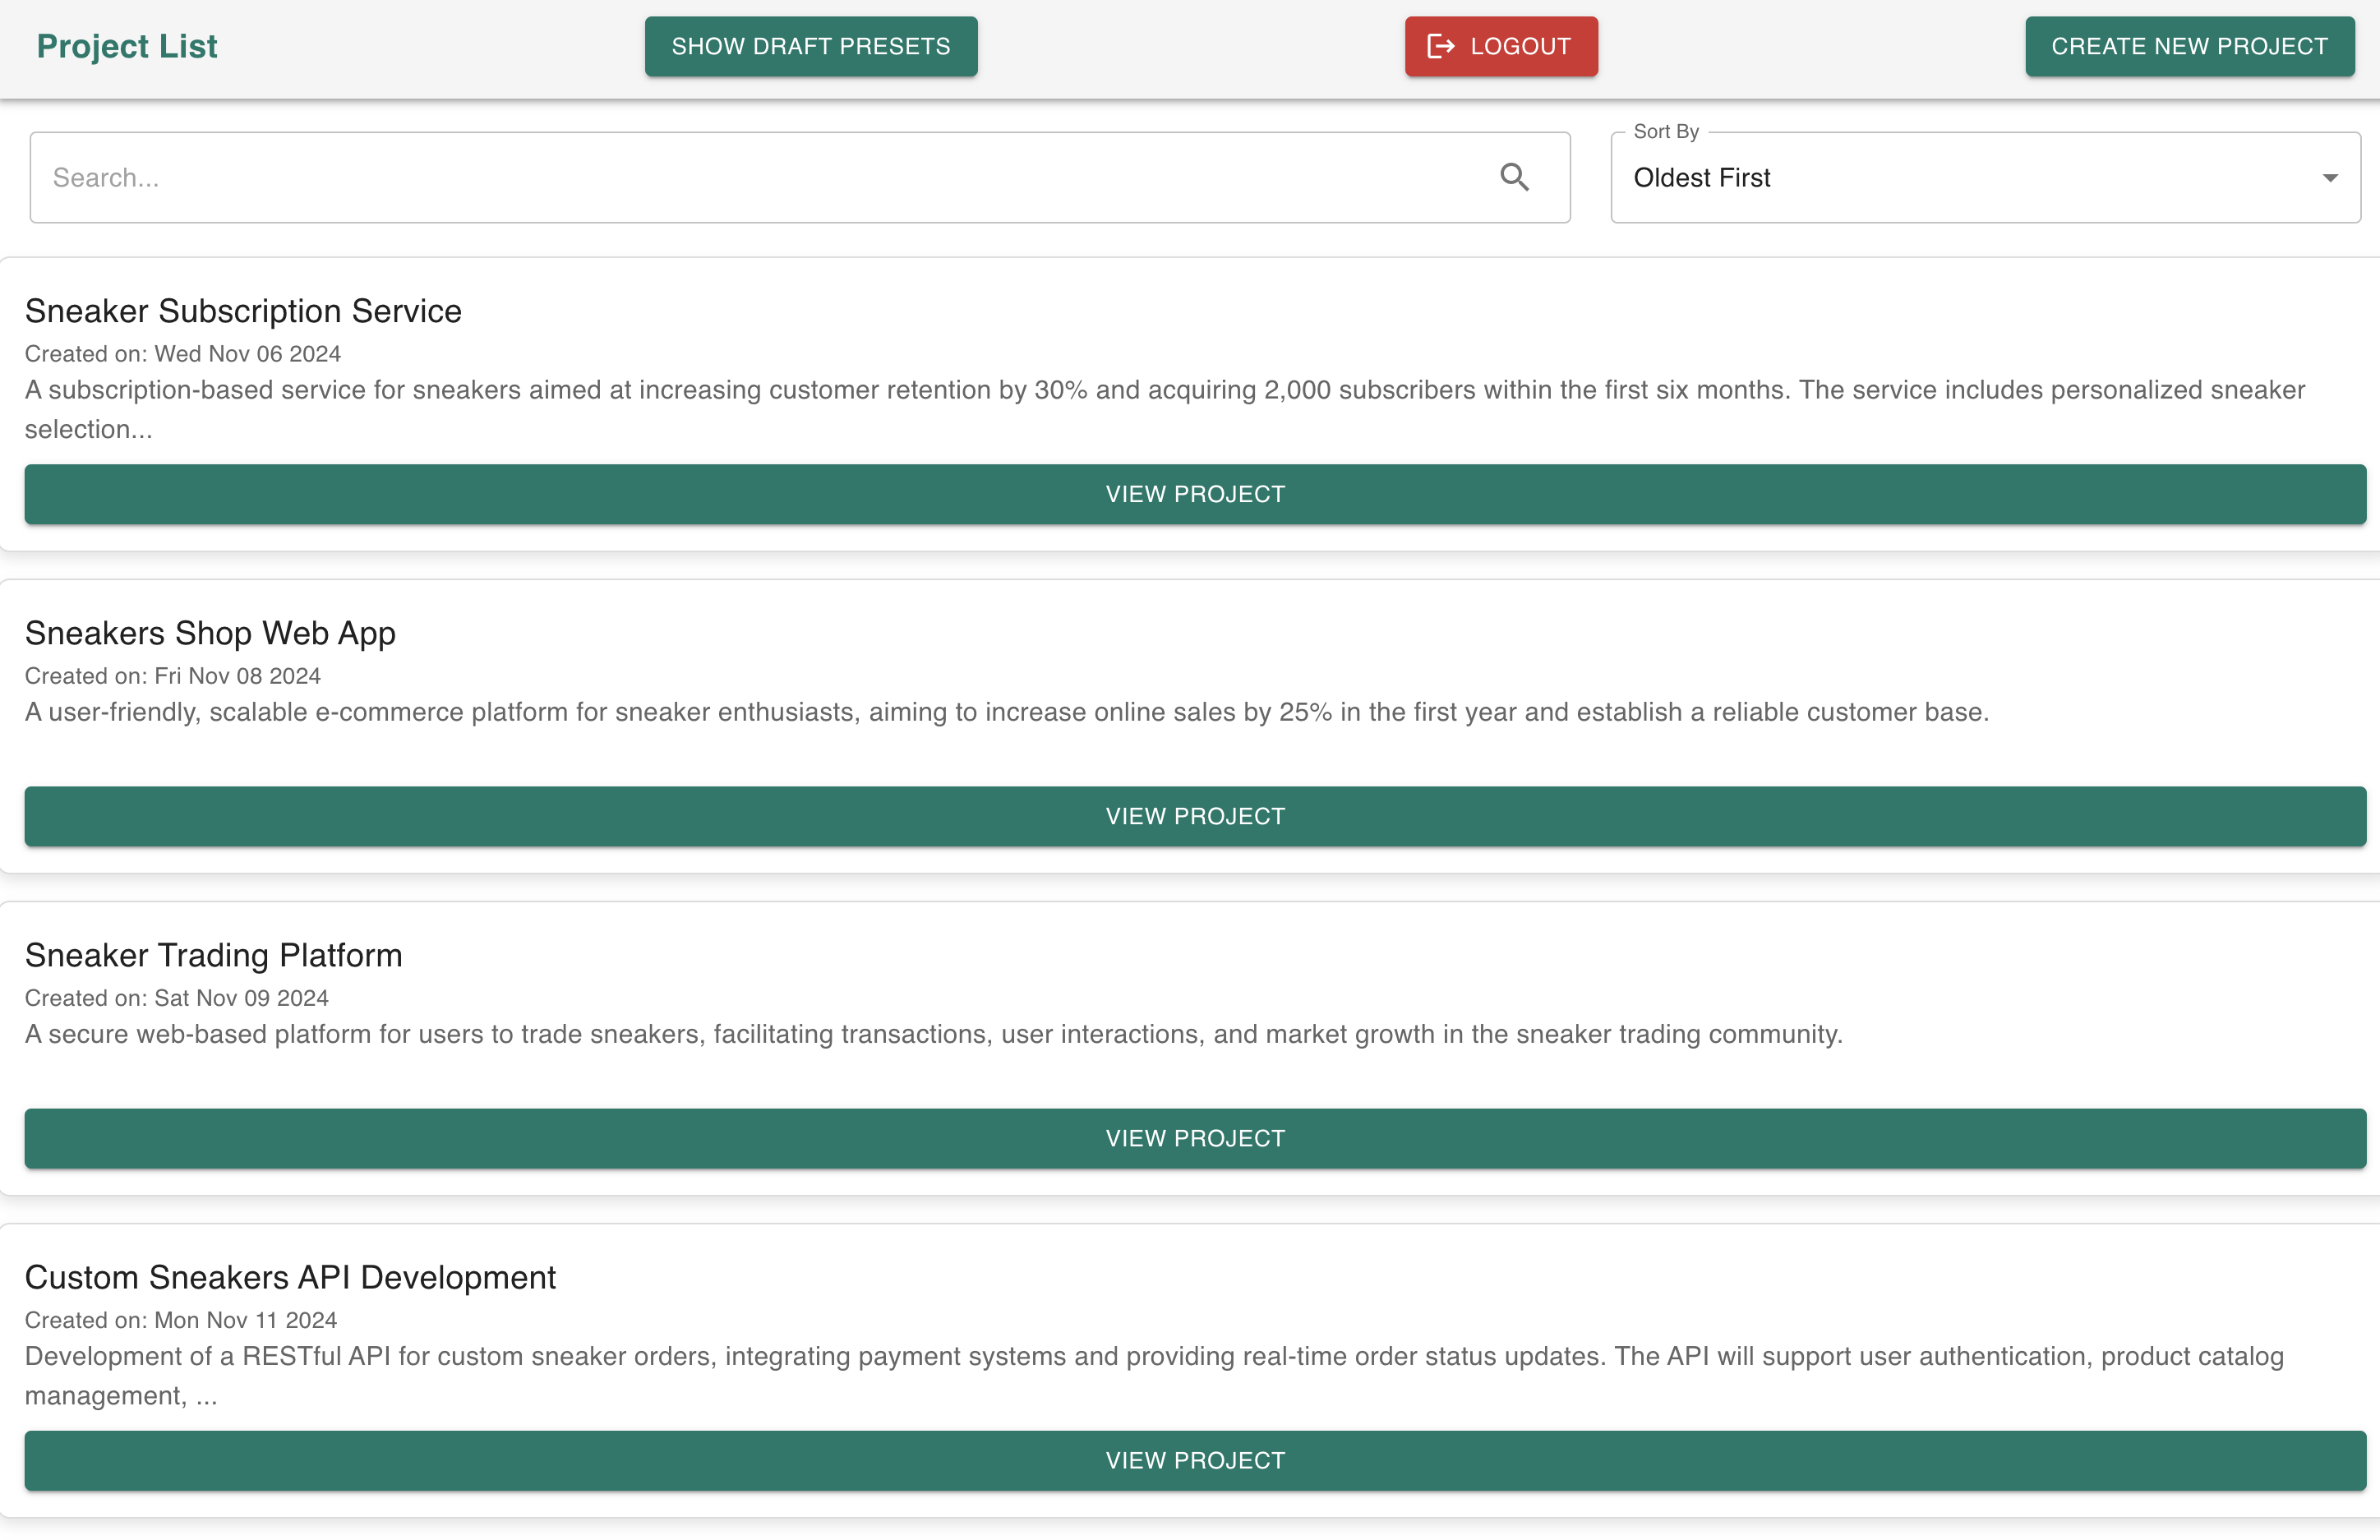
\includegraphics[width=1\textwidth]{applicazione/dashboard.png}
    \caption{Schermata della \textit{dashboard} del progetto}
    \label{fig:dashboard}
\end{figure}

\pagebreak
\noindent La {\hyperref[fig:create-project]{Figura 3.8}} riporta la pagina di generazione di un progetto che permette di creare nuovi progetti inserendo il nome, selezionando un \textit{preset} e completandolo in tutte le sue sezioni.\\
Una volta compilato, l’utente può procedere con la generazione del progetto. \\
È inoltre possibile salvare il \textit{preset} parzialmente compilato come bozza per riprendere la sua compilazione in un secondo momento.
\begin{figure}[H]
    \centering
    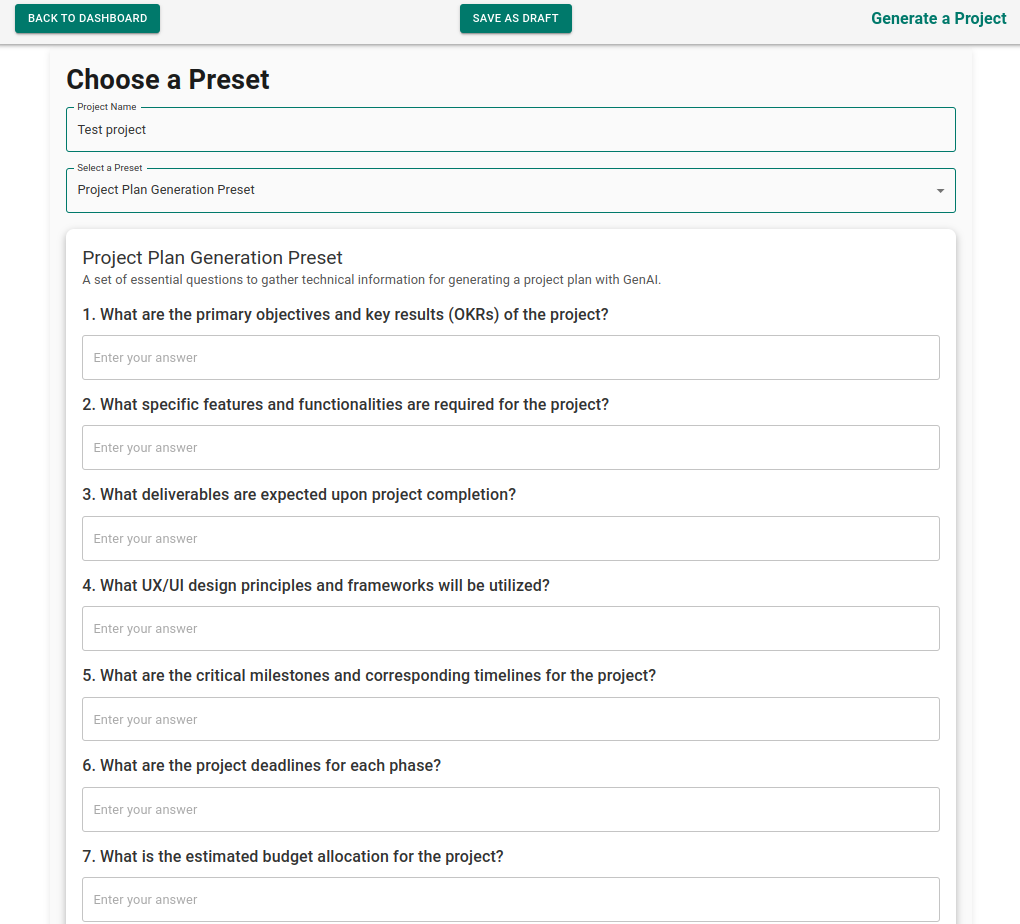
\includegraphics[width=1\textwidth]{applicazione/create-project.png}
    \caption{Schermata di generazione del progetto}
    \label{fig:create-project}
\end{figure}

\pagebreak
\noindent La {\hyperref[fig:project-detail]{Figura 3.9}} mostra la pagina di visualizzazione di un singolo progetto che offre una descrizione completa di tutte le informazioni relative al progetto, inclusi i dettagli tecnici ed il PDF generato, che può essere visualizzato direttamente nella pagina. \\ 

\noindent Inoltre gli utenti possono scegliere di rigenerare l’intero progetto o una singola sezione, utilizzando una finestra che consente di inserire un \gls{prompt} personalizzato, come riporta la {\hyperref[fig:regenerate-project]{Figura 3.10}}.\\
\begin{figure}[H]
    \centering
    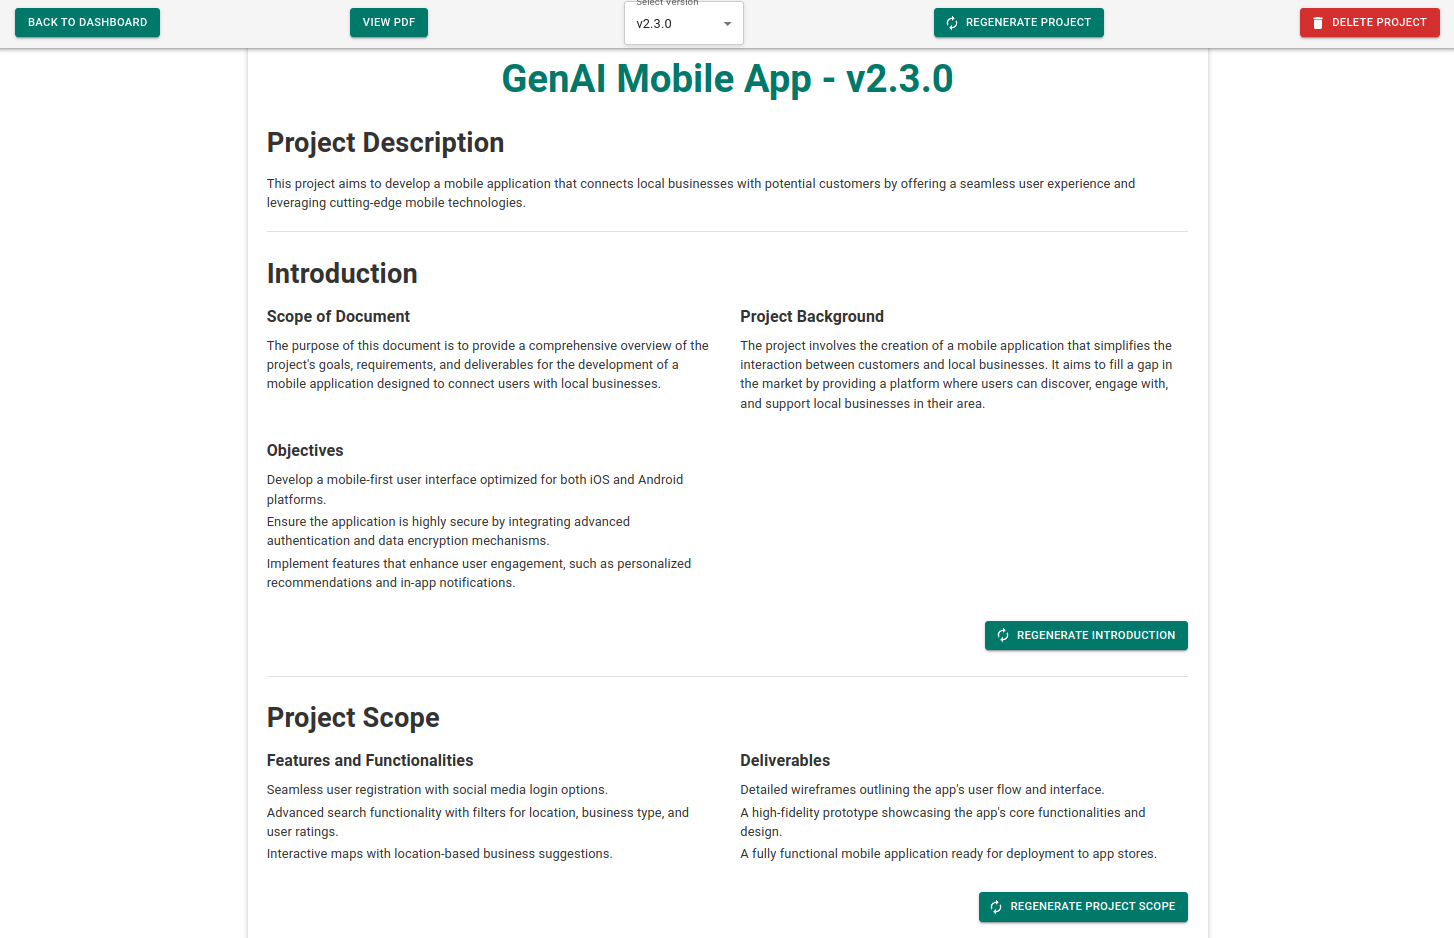
\includegraphics[width=1\textwidth]{applicazione/project-detail.png}
    \caption{Schermata di dettaglio del progetto}
    \label{fig:project-detail}
\end{figure}

\begin{figure}[H]
    \centering
    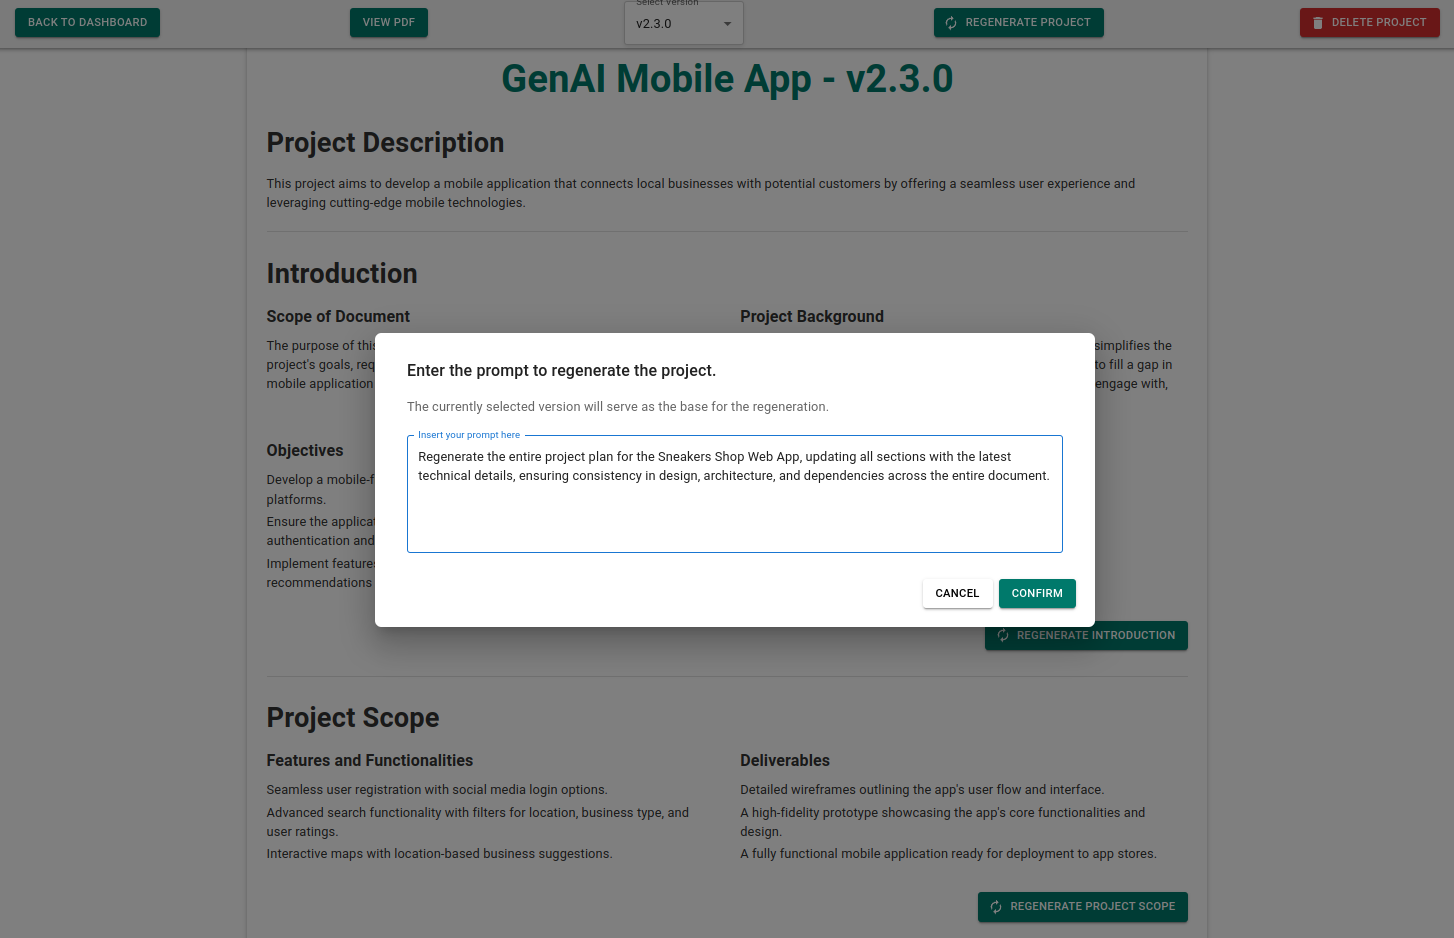
\includegraphics[width=1\textwidth]{applicazione/regenerate-project.png}
    \caption{\gls{prompt} per rigenerare il progetto}
    \label{fig:regenerate-project}
\end{figure}

\pagebreak
\noindent Infine la {\hyperref[fig:swagger]{Figura 3.11}} riporta la pagina di visualizzazione del \textit{Swagger} delle \gls{api}, essa fornisce una documentazione interattiva e dettagliata delle \gls{api} disponibili nel sistema. \\
Attraverso questa pagina, gli utenti possono esplorare i vari \textit{endpoint}, visualizzarne le descrizioni, i parametri richiesti e le risposte previste. \\
Inoltre, è possibile effettuare chiamate di prova direttamente dalla pagina, inserendo i parametri necessari e verificando i risultati in tempo reale. 
\begin{figure}[H]
    \centering
    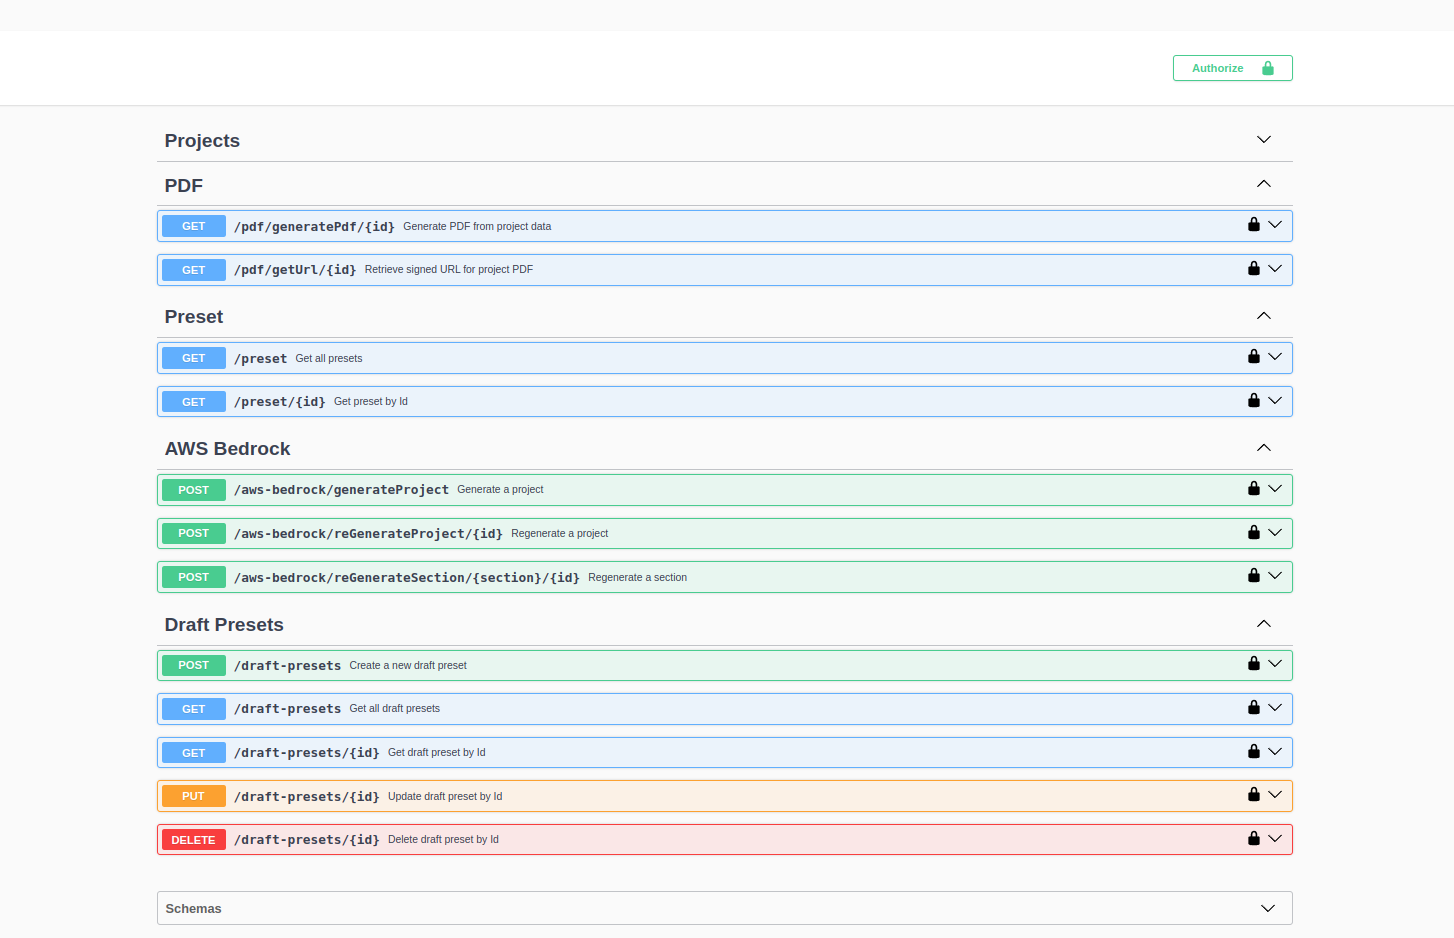
\includegraphics[width=1\textwidth]{applicazione/swagger.png}
    \caption{\textit{Swagger} delle \gls{api} create}
    \label{fig:swagger}
\end{figure}